%----------------------------------------------------------------------------------------------------=
%-----------------------------------------------------------------------------------------------------
% Define Document Class, and include/import the multiple libraries used to create this document 
%-----------------------------------------------------------------------------------------------------
\documentclass[12pt]{article}
\usepackage{amsmath}
\usepackage[sc]{mathpazo}
\usepackage{geometry}
\usepackage{datetime}
\usepackage[myheadings]{fullpage}
\usepackage{fancyhdr}
\usepackage{lastpage}
\usepackage{graphicx, wrapfig, subcaption, setspace, booktabs}
\usepackage[T1]{fontenc}
\usepackage[font=small, labelfont=bf]{caption}
\usepackage{fourier}
\usepackage[protrusion=true, expansion=true]{microtype}
\usepackage[english]{babel}
\usepackage{sectsty}
\usepackage{url, lipsum}
\usepackage{hyperref,bookmark}
\usepackage[T1]{fontenc}
\usepackage{amssymb}
\usepackage{listings}
\usepackage{xcolor}
\usepackage{tabularx}
\usepackage{longtable}
\usepackage{setspace}
\usepackage{float}
\usepackage{bigfoot} % to allow verbatim in footnote
\usepackage[framed,numbered,autolinebreaks,useliterate]{matlab-prettifier}
\usepackage{filecontents}
\usepackage[ruled,linesnumbered]{algorithm2e}

%-----------------------------------------------------------------------------------------------------
% Define the heading for this document
%-----------------------------------------------------------------------------------------------------
% Heading style, calling fancy header library
\pagestyle{fancy}
\fancyhf{}
\setlength\headheight{15pt}
%%%% PUT YOUR NAME HERE FOR YOUR HEADING %%%%
\fancyhead[L]{Luis Fernando Enriquez-Contreras}
\fancyhead[R]{EE 105 Lab 2 Solution}
\fancyfoot[R]{Page \thepage\ of \pageref{LastPage}}

%-----------------------------------------------------------------------------------------------------
% Set coding for in LaTeX for Matlab
%-----------------------------------------------------------------------------------------------------
\lstset{
	style              = Matlab-editor,
	basicstyle         = \mlttfamily,
	escapechar         = ",
	mlshowsectionrules = true,
	otherkeywords = {!,!=,~,$,*,\&,\%/\%,\%*\%,\%\%,<-,<<-,_,/},%
}

% The workflow of the document begins here
\begin{document}
	%-------------------------------------------------------------------------------
	% Title
	%-------------------------------------------------------------------------------
	\begin{titlepage}
		
		\newcommand{\HRule}{\rule{\linewidth}{0.5mm}} % Defines a new command for the horizontal lines, change thickness here
		
		\center % Center everything on the page
		
		%---------------------------------------------------------
		%	HEADING SECTIONS
		%---------------------------------------------------------
		
		\textsc{\LARGE University of California, Riverside}\\[1.5cm] % Name of your university/college
		\textsc{\Large Bourns College of Engineering}\\[0.5cm] % Major heading such as course name
		\textsc{\large Department of Electrical and Computer Engineering}\\[0.5cm] % Minor heading such as course title
		
		%---------------------------------------------------------
		%	TITLE SECTION
		%---------------------------------------------------------
		
		\HRule \\[0.6cm]
		{\Large EE 105 Lab 2 Solution \\ \normalsize Euler's}\\[0.4cm] % Title of your document
		\HRule \\[1.0cm]
		
		%---------------------------------------------------------
		%	AUTHOR SECTION
		%---------------------------------------------------------
		
		%\begin{minipage}{0.4\textwidth}
		\begin{center} \large
			% \emph{Authors:}  
			\medskip
			%%% PUT YOUR NAME HERE %%%
			{\textsc{\textbf{Luis Fernando Enriquez-Contreras} }} 
		\end{center}
		%\end{minipage}
		
		
		%---------------------------------------------------------
		%	DATE SECTION
		%---------------------------------------------------------
		\begin{center}
			%			\selectlanguage{USenglish}
			{\large }
		\end{center}
		% Date, change the \today to a set date if you want to be precise
		
		%---------------------------------------------------------
		%	LOGO SECTION
		%---------------------------------------------------------
		%\vfill
		\newcommand*{\plogo}{
\includegraphics{Code/Fig/UC_Riverside_seal.pdf}}
		%		\newcommand*{\plogo}{
\includegraphics[width=0.25\textwidth]{UC_Riverside_seal.pdf}}
		
		\plogo\\[1cm] % Include a department/university logo - this will require the graphicx package
		
		%---------------------------------------------------------
		
		\vfill % Fill the rest of the page with whitespace
	\end{titlepage}
	
	\newpage
	
	%-------------------------------------------------------------------------------
	% Table of Contents and Figures
	%-------------------------------------------------------------------------------
	%	\doublespacing
	\tableofcontents
	\pagebreak
	\listoffigures
	\listoftables
	\lstlistoflistings  
	\pagebreak
	
	%-------------------------------------------------------------------------------
	% BODY
	%-------------------------------------------------------------------------------
	
	\section{Introduction}
	%%% PUT INTRODUCTION HERE %%%
	This laboratory exercise aims to equip you with a firm understanding of the practicalities and potential challenges associated with numerically solving differential equations. Through hands-on simulations using MATLAB, you'll gain valuable experience in modeling and analyzing dynamic systems.
	
	\subsection{Objectives}
	\begin{itemize}
		\item Master the concepts: Gain a comprehensive understanding of the key principles and methods involved in numerical differential equation solvers
		\item Develop simulation skills: Learn how to leverage MATLAB's capabilities to construct simulations of dynamic systems accurately and efficiently
		\item Identify potential pitfalls: Be aware of common issues and limitations that can arise when solving differential equations numerically, enabling you to approach numerical solutions with prudence and insight
		\item Apply your knowledge: Put your newfound skills into practice by constructing and analyzing your own dynamic system simulation in MATLAB
	\end{itemize}
	
	\section{Pre-Lab}
		Given the transfer function:
		
		$$
		H(s)=\frac{36}{s^{2}+3 s+36}
		$$
		
		We can determine the following values:
		
		$$
		\begin{aligned}
			\omega_{n} & =6 \\
			G & =1 \\
			\zeta & =\frac{3}{12} = \frac{1}{4}  \\
			\sigma & =\zeta \omega_{n}= \frac{6}{4} = 1.5\\
			\omega_{d} & =\omega_{n} \sqrt{1-\zeta} \approx 5.2
		\end{aligned}
		$$
		$$
		\begin{aligned}
			T_r=\frac{1.8}{\omega_n} \ &
			T_p=\frac{\pi}{\omega_{d}} \  &
			T_s=\frac{4.6}{\sigma} \ &
			M_p(\zeta) = e^{\frac {- \zeta \pi }{\sqrt{1-\zeta^{2}}}}
		\end{aligned}
		$$
		$$
		\begin{aligned}
			T_r= 0.3 \ &
			T_p \approx 0.60384 \ &
			T_s = 3.066\overline{6} \ &
			M_p(\zeta) \approx 0.4329
		\end{aligned}
		$$
		The steady state response is given by:
		
		$$
		\begin{aligned}
			H(s) & =\frac{36}{s^{2}+3 s+36} \\
			\left.H(s)\right|_{s=j \omega} & =\frac{36}{36-\omega^{2}+3 j \omega} \\
			|H(j \omega)|^{2} & =H(j \omega) H(j \omega)^{*} \\
			& =\left(\frac{36}{36-\omega^{2}+3 j \omega}\right)\left(\frac{36}{36-\omega^{2}-3 j \omega}\right) \\
			|H(j \omega)| & =\frac{36}{\sqrt{\left(\left(36-\omega^{2}\right)^{2}+9 \omega^{2}\right)}}  \approx 1.0002\\
			\angle H(j \omega) & =\left(\frac{36}{36-\omega^{2}+3 j \omega}\right)\left(\frac{36-\omega^{2}-3 j \omega}{36-\omega^{2}-3 j \omega}\right) \\
			& =\frac{36\left(36-\omega^{2}-3 j \omega\right)}{\left(36-\omega^{2}\right)^{2}-9 \omega^{2}} = 0.7856^{\circ}
		\end{aligned}
		$$
		
		The steady state response is given by the following:
		
		$$
		y(t)=1.0002 \sin \left(0.1 t-0.7856^{\circ}\right)
		$$
		
		Given that $x=\left[\begin{array}{ll}y & \dot{y}\end{array}\right]^{T}$
		
		$$
		\begin{aligned}
			\dot{x}_{1} & =x_{2} \\
			\dot{x}_{2} & =\ddot{y}(t) \\
			\frac{Y(s)}{U(s)} & =\frac{36}{s^{2}+3 s+36} \\
			Y(s)\left(s^{2}+3 s+36\right) & =36 U(s) \\
			s^{2} Y(s)+3 s Y(s)+36 Y(s) & =36 U(s) \\
			\mathcal{L}^{-1}\left[s^{2} Y(s)+3 s Y(s)+36 Y(s)\right] & =\mathcal{L}^{-1}[36 U(s)] \\
			\ddot{y}(t)+3 \dot{y}(t)+36 y(t) & =36 u(t) \\
			\ddot{y}(t) & =36 u(t)-3 \dot{y}(t)-36 y(t) \\
			\ddot{y}(t) & =36 u(t)-3 x_{2}-36 x_{1} \\
			\dot{x}_{2} & =36 u(t)-3 x_{2}-36 x_{1} \\
			\dot{x} & =\left[x_{2}; 36 u(t)-3 x_{2}-36 x_{1}\right] \\
			y & =\left[x_{1}\right]
		\end{aligned}
		$$
		
		The system is linear, therefore we can solve for $A, B, C, D$
		
		$$
		\begin{array}{ll}
			A=\left[\begin{array}{cc}
				0 & 1 \\
				-36 & -3
			\end{array}\right] & B=\left[\begin{array}{c}
				0 \\
				36
			\end{array}\right] \\
			C=\left[\begin{array}{ll}
				1 & 0
			\end{array}\right] & D=[0]
		\end{array}
		$$
	\section{LSIM and gensig}
		%%% INSERT CODE HERE AS A .m FILE %%%
		\lstinputlisting[language=Matlab, caption = {\Large lsim Simulation of the State Space Model with domain of 0-100 seconds}]{Code/lsim_run_100.m}
		%%% INSERT CODE HERE AS A .m FILE %%%
		\lstinputlisting[language=Matlab, caption = {\Large lsim Simulation of the State Space Model with domain of 0-4 seconds}]{Code/lsim_run_4.m}
		
		%%% Insert Figure Here as a .pdf File %%%
		\begin{figure}[H]
			\centering
			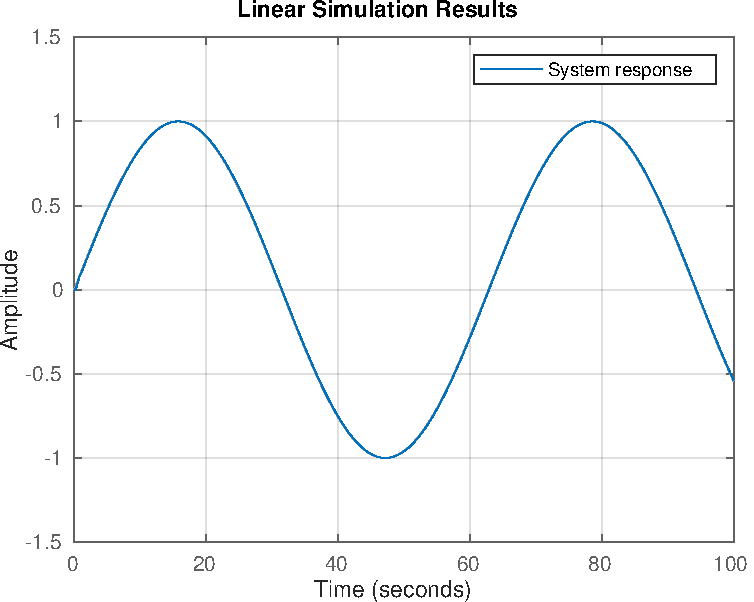
\includegraphics[width=1\linewidth]{"Code/Fig/lsim_run_100s.pdf"}
			\caption{lsim Simulation of the State Space Model with a domain of 0-100 seconds}
			\label{fig:lsimrun100s}
		\end{figure}
		%%% Insert Figure Here as a .pdf File %%%
		\begin{figure}[H]
			\centering
			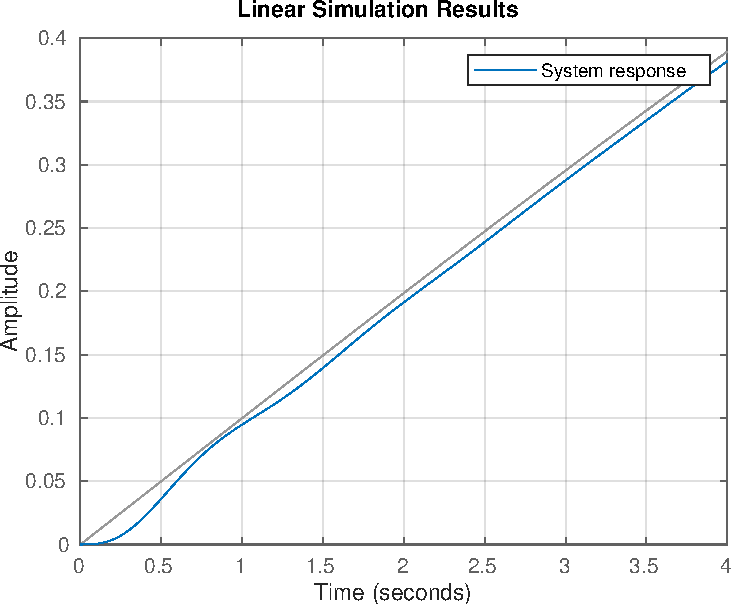
\includegraphics[width=1\linewidth]{"Code/Fig/lsim_run_4s.pdf"}
			\caption{lsim Simulation of the State Space Model with a domain of 0-4 seconds}
			\label{fig:lsimrun4s}
		\end{figure}

	\section{Varying Step-Size of 1.0 sin(0.1)}
		%%% INSERT CODE HERE AS A .m FILE %%%
		\lstinputlisting[language=Matlab, caption = {\Large Function for the State Space of the representation of the system}]{Code/f.m}
		
		%%% INSERT CODE HERE AS A .m FILE %%%
		\lstinputlisting[language=Matlab, caption = {\Large Function to run Euler recursion}]{Code/Euler.m}
		
		%%% INSERT CODE HERE AS A .m FILE %%%
		\lstinputlisting[language=Matlab, caption = {\Large Run the Euler function for different step sizes $h$}]{Code/run_Euler.m}
		%%% Insert Figure Here as a .pdf File %%%
		\begin{figure}[H]
			\centering
			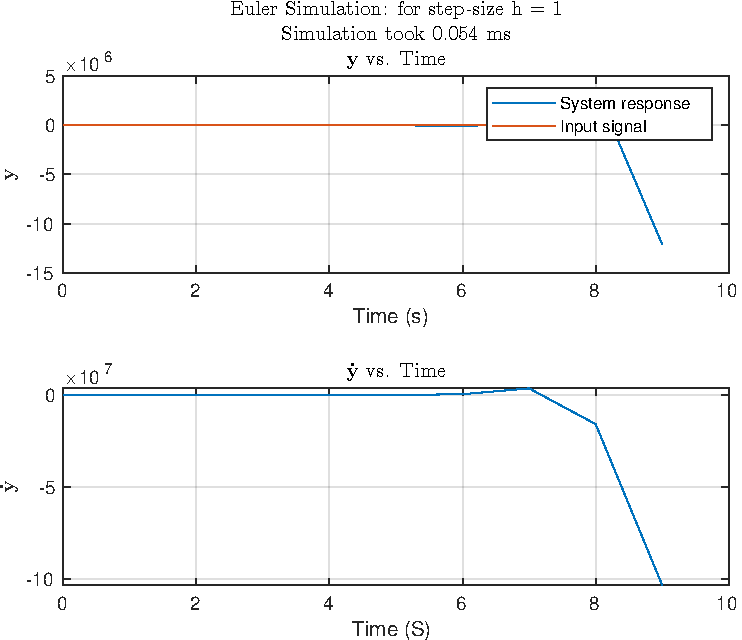
\includegraphics[width=1\linewidth]{"Code/Fig/Euler_plot_h_1.pdf"}
			\caption{Euler Plot for $h$ = 1}
			\label{fig:eulerploth1}
		\end{figure}	
		%%% Insert Figure Here as a .pdf File %%%
		\begin{figure}[H]
			\centering
			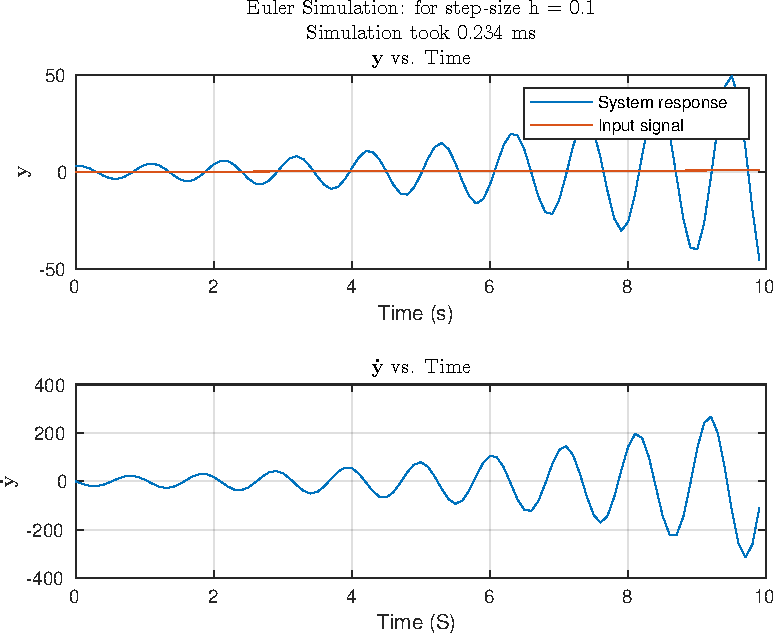
\includegraphics[width=1\linewidth]{"Code/Fig/Euler_plot_h_0.1.pdf"}
			\caption{Euler Plot for $h$ = 0.1}
			\label{fig:eulerploth01}
		\end{figure}
		%%% Insert Figure Here as a .pdf File %%%
		\begin{figure}[H]
			\centering
			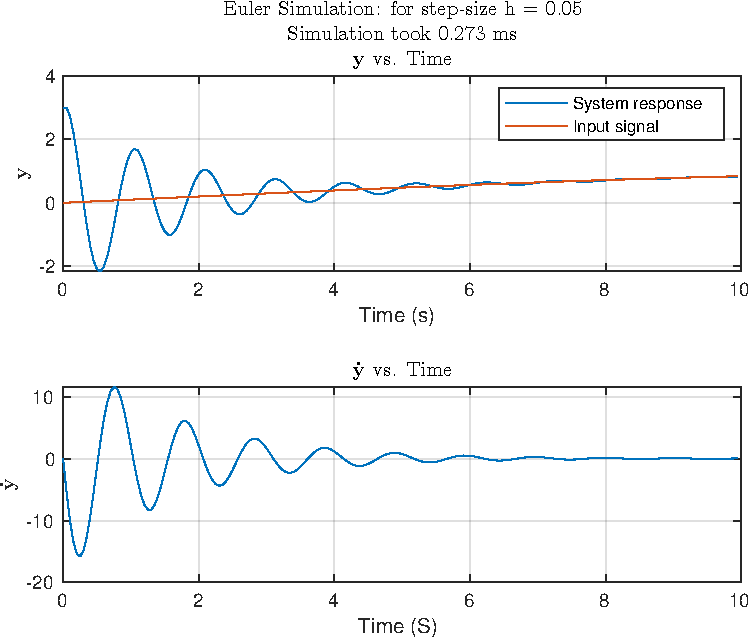
\includegraphics[width=1\linewidth]{"Code/Fig/Euler_plot_h_0.05.pdf"}
			\caption{Euler Plot for $h$ = 0.05}
			\label{fig:eulerploth005}
		\end{figure}
		
		\begin{figure}[H]
			\centering
			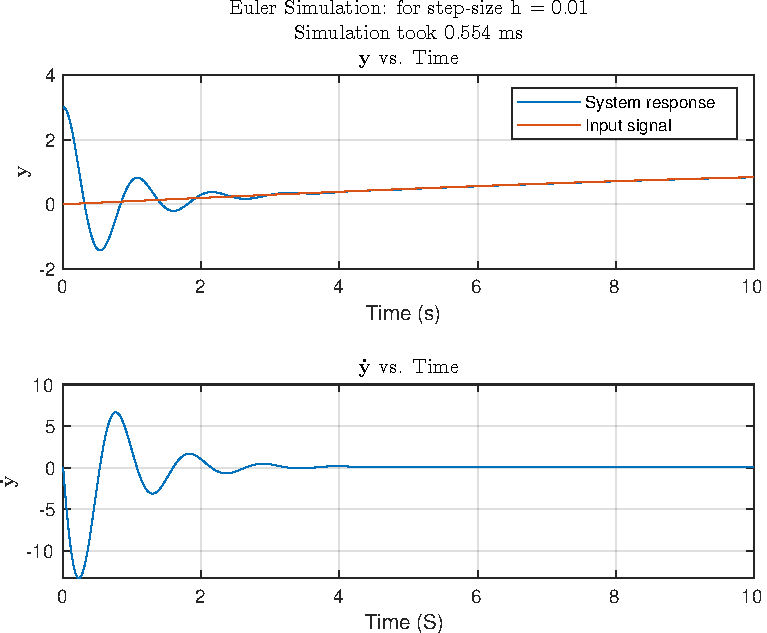
\includegraphics[width=1\linewidth]{"Code/Fig/Euler_plot_h_0.01.pdf"}
			\caption{Euler Plot for $h$ = 0.01}
			\label{fig:eulerploth001}
		\end{figure}
		%%% Insert Figure Here as a .pdf File %%%
		\begin{figure}[H]
			\centering
			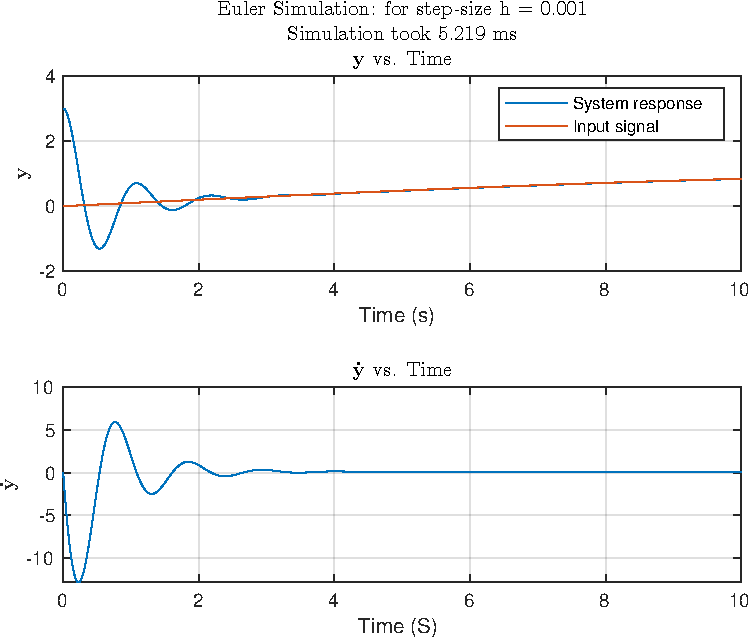
\includegraphics[width=1\linewidth]{"Code/Fig/Euler_plot_h_0.001.pdf"}
			\caption{Euler Plot for $h$ = 0.001}
			\label{fig:eulerploth0001}
		\end{figure}
	
		Figures \ref{fig:eulerploth1}, \ref{fig:eulerploth01} do not settle at all. Figure \ref{fig:eulerploth005} does settle, but does so at around 7-8 seconds. Figures \ref{fig:eulerploth001}, \ref{fig:eulerploth0001} do settle at around 3 seconds which is close to $T_{S}$ calculated. 
		\begin{table}[H]
			\centering
			\caption{Cputimes for Various Euler's Step Sizes}
			\begin{tabular}{|c|r|r|r|r|r|r|r|r|}
				\hline & \multicolumn{2}{|c|}{$h=1.0 \mathrm{~s}$} & \multicolumn{2}{c|}{$h=0.1 \mathrm{~s}$} & \multicolumn{2}{c|}{$h=0.01 \mathrm{~s}$} & \multicolumn{2}{|c|}{$h=0.001 \mathrm{~s}$} \\
				\hline Time, $t$ & $k$ & $x_k$ & $k$ & $x_k$ & $k$ & $x_k$ & $k$ & $x_k$ \\
				\hline 0.0 & 0 & 3 & 0 & 3 & 0 & 3 & 0 & 3 \\
				2.0 & 2 & 3 & 20 & 0.9790 & 200 & 0.289 & 2000 & 0.2508 \\
				4.0 & 4 & 6.5940 & 40 & -3.6305 & 400 & 0.3764 & 4000 & 0.3775 \\
				6.0 & 6 & -3784.1155 & 60 & -14.03887 & 600 & 0.5561 & 6000 & 0.5574 \\
				8.0 & 8 & 3752170.88274 & 80 & -30.2920 & 800 & 0.7109 & 8000 & 0.7116\\
				10.0 & 10 & -12125600.5695 & 100 & -45.5193 & 1000 & 0.8366 & 10000 & 0.8371 \\
				\hline CPUTIME (ms) & & 0.054 & & 0.234 & & 0.554 & & 5.219 \\
				\hline
			\end{tabular}
		\end{table}
	\section{ODE23 with Zero Input}
	
		\begin{figure}[H]
			\centering
			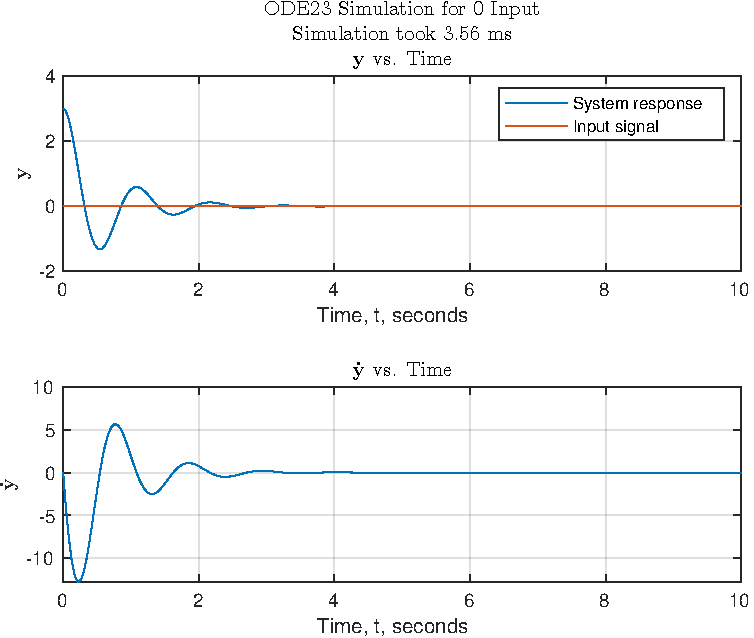
\includegraphics[width=1\linewidth]{Code/Fig/ode_no_input}
			\caption{ODE Plot for Zero Input}
			\label{fig:odenoinput}
		\end{figure}
		
					
	\section{Varying $\omega$ in 1.0 sin($\omega$t)}
		%%% INSERT CODE HERE AS A .m FILE %%%
		\lstinputlisting[language=Matlab, caption = {\Large Function for the State Space of the representation of the system for ODE23}]{Code/f_ode.m}
		
		%%% INSERT CODE HERE AS A .m FILE %%%
		\lstinputlisting[language=Matlab, caption = {\Large Run ODE23 for sin(0.1t)}]{Code/ode_sin_input.m}
		
		\begin{figure}[H]
			\centering
			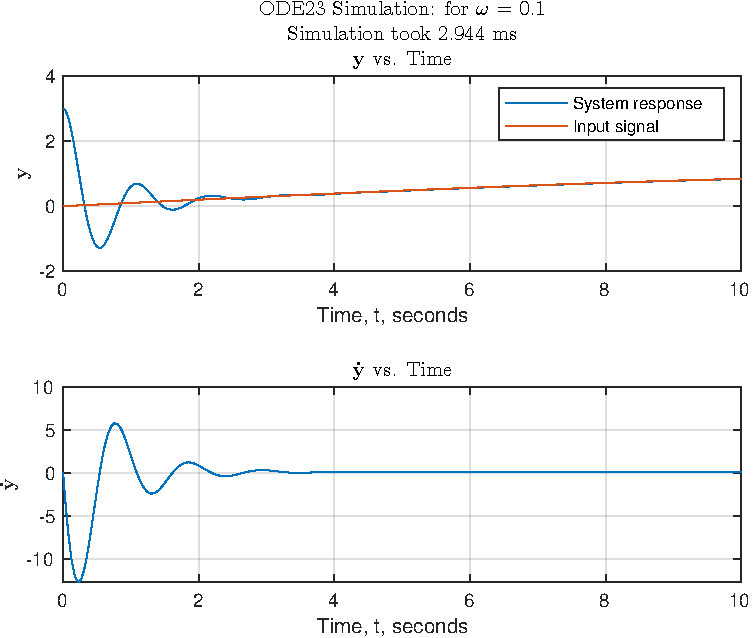
\includegraphics[width=1\linewidth]{Code/Fig/ode_sin_input_0.1}
			\caption{Ode Plot for $\omega$ = 0.1}
			\label{fig:odesininput0}
		\end{figure}
		
		
		%%% INSERT CODE HERE AS A .m FILE %%%
		\lstinputlisting[language=Matlab, caption = {\Large Run ODE23 for various sin($\omega$t)}]{Code/ode_sin_input_omega.m}	
		%%% Insert Figure Here as a .pdf File %%%
		\begin{figure}[H]
			\centering
			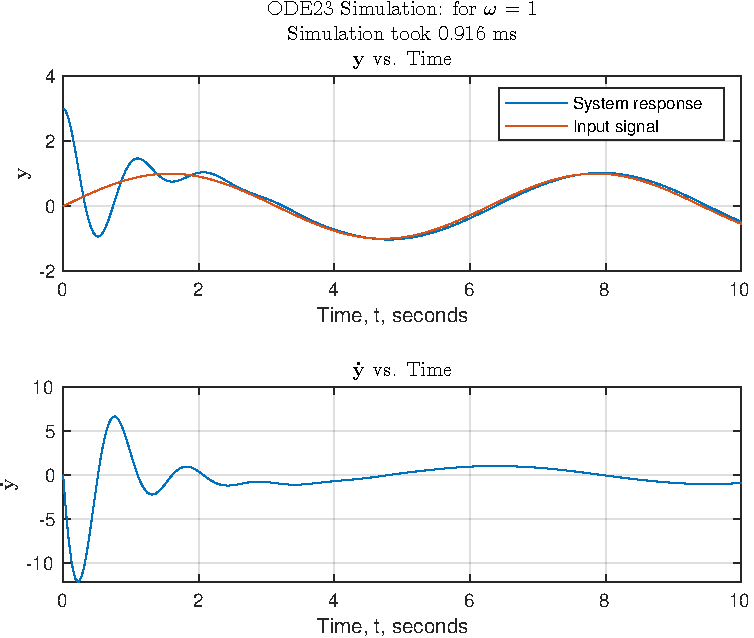
\includegraphics[width=1\linewidth]{Code/Fig/ode_sin_input_1}
			\caption{Ode Plot for $\omega$ = 1}
			\label{fig:odesininput1}
		\end{figure}
		%%% Insert Figure Here as a .pdf File %%%
		\begin{figure}[H]
			\centering
			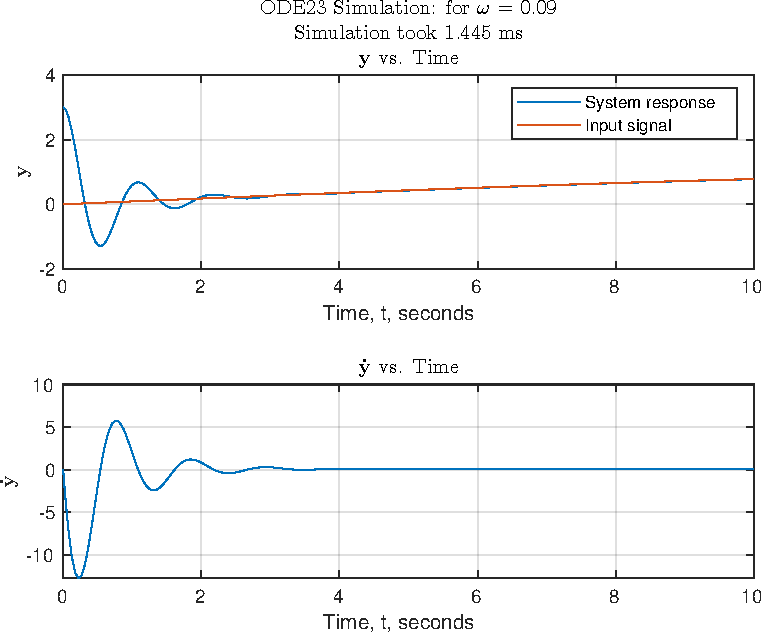
\includegraphics[width=1\linewidth]{Code/Fig/ode_sin_input_0.09}
			\caption{Ode Plot for $\omega$ = 0.09}
			\label{fig:odesininput009}
		\end{figure}
		%%% Insert Figure Here as a .pdf File %%%
		\begin{figure}[H]
			\centering
			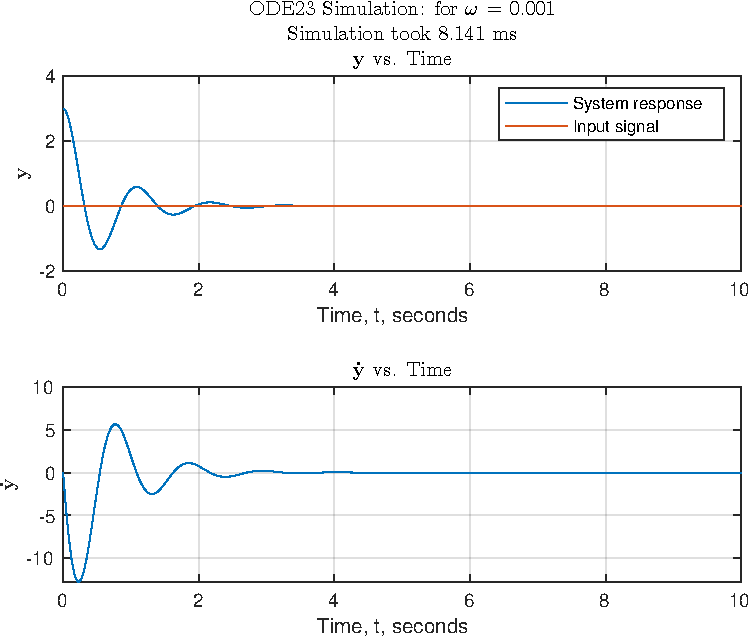
\includegraphics[width=1\linewidth]{Code/Fig/ode_sin_input_0.001}
			\caption{Ode Plot for $\omega$ = 0.001}
			\label{fig:odesininput0001}
		\end{figure}		
	
		\subsection{Bode Plot}
	
		%%% INSERT CODE HERE AS A .m FILE %%%
		\lstinputlisting[language=Matlab, caption = {\Large Bode Plot Code for State Space Function}]{Code/bode.m}
		
		\begin{figure}[H]
			\centering
			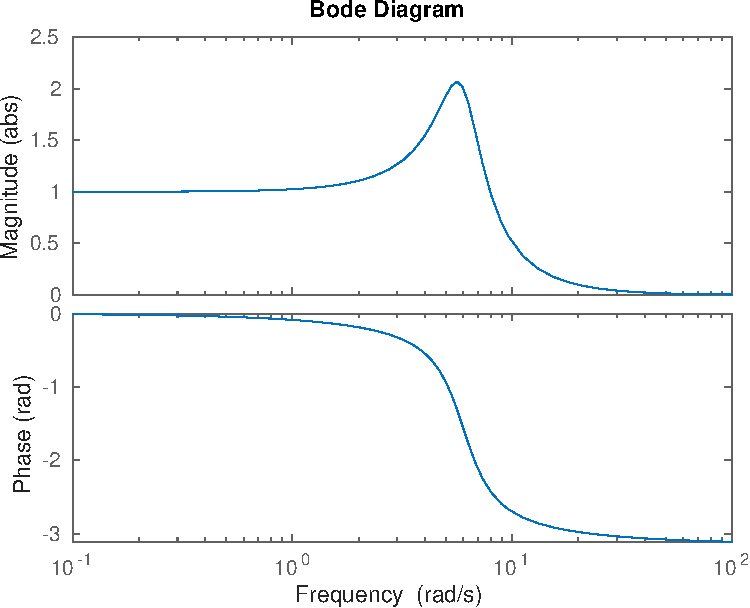
\includegraphics[width=1\linewidth]{Code/Fig/bode_plot}
			\caption{Bode Plot for State Space Model}
			\label{fig:bodeplot}
		\end{figure}
	
		\begin{itemize}
			\item At $\omega$ = 1, the amplitude is 1.02481 and the phase is -0.0855053
			\item At $\omega$ = 0.09, the amplitude is 1.0002 and the phase is -0.00750155
			\item At $\omega$ = 0.001, the amplitude is 1 and the phase is -8.33333e-05
		\end{itemize}
		
	\section{Conclusion}
	%%% PUT CONCLUSION HERE %%
	This MATLAB lab successfully explored the intricacies and challenges of numerically solving differential equations. By constructing a dynamic system simulation, we gained practical experience in applying various numerical methods and interpreting the results.
	
	\begin{itemize}
		\item Students solidified our understanding of how numerical methods approximate the solution of differential equations
		\item Students explored different MATLAB tools and techniques for implementing these methods, such as ode23 and custom functions
		\item Students learned to critically evaluate the accuracy and stability of numerical solutions, considering factors like step size and tolerance
		\item Students became aware of potential pitfalls like stiffness and convergence issues, highlighting the importance of choosing appropriate methods and parameter values
	\end{itemize}
	
\end{document}